%!Mode:: "TeX:UTF-8"
\section{计算机体系结构}

\textbf{冯·诺依曼结构}也称\textbf{普林斯顿}结构,是一种将程序指令存储器和数据存储器合并在一起的存储器结构。程序指令存储地址和数据存储地址指向同一个存储器的不同物理位置,因此程序指令和数据的宽度相同,如英特尔公司的8086中央处理器的程序指令和数据都是16位宽。


\textbf{哈佛结构}是一种将程序指令存储和数据存储分开的存储器结构,即程序存储器和数据存储器是两个独立的存储器,每个存储器独立编址、独立访问。与两个存储器相对应的是系统的4条总线:程序的数据总线与地址总线,数据的数据总线与地址总线。这种分离的程序总线和数据总线可允许在一个机器周期内同时获得指令字(来自程序存储器)和操作数(来自数据存储器)。程序指令存储和数据存储分开,可以使指令和数据有不同的数据宽度。哈佛结构是为了高速数据处理而采用的,因为可以同时读取指令和数据(分开存储的)。大大提高了数据吞吐率,缺点是结构复杂。


\begin{figure}[ht]
	\begin{center}
	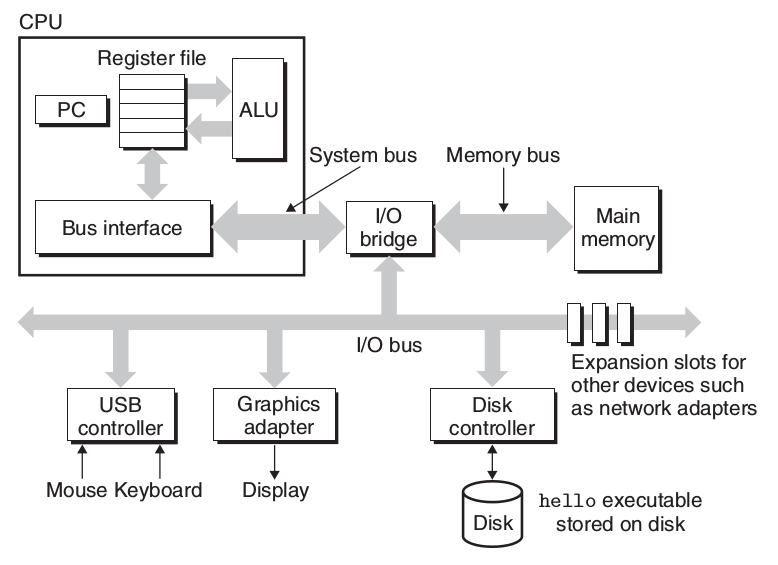
\includegraphics[keepaspectratio,width=0.3\paperwidth]{Pictures/sysBusCsapp.png}
		\caption{CSAPP:硬件体系结构}
	\label{fig:HardwareStructure}
	\end{center}
\end{figure}

\textbf{改进的哈佛结构},其结构特点为:
使用两个独立的存储器模块,分别存储指令和数据,每个存储模块都不允许指令和数据并存,以便实现并行处理;具有一条独立的地址总线和一条独立的数据总线,利用\textbf{公用地址总线}访问两个存储模块(程序存储模块和数据存储模块),\textbf{公用数据总线}则被用来完成程序存储模块或数据存储模块与CPU之间的数据传输;两条总线由程序存储器和数据存储器分时共用。

x86-64(简称x64)是64位版本的x86指令集,向前兼容于16位及32位的x86架构。x64于1999年由AMD设计,AMD首次公开64位集以扩充给x86,称为“AMD64”。其后也为英特尔所采用,现时英特尔称之为“Intel 64”,在之前曾使用过“Clackamas Technology” (CT)、“IA-32e”及“EM64T”。
Apple使用"x86-64"去称呼此64位架构。太阳微系统(已被甲骨文收购)及Microsoft称它为"x64"。BSD家族及其他Linux发布版则使用"amd64",32位版本则称为"i386"(或i486/586/686)。

\clearpage